% Ensure that you compile using XeLaTeX !!! PDFTex has problems with some of the packages used
\documentclass[12pt]{article}
\setlength\parindent{0pt}

\usepackage{parskip}
\usepackage[margin=0.5in]{geometry}
\usepackage{fullpage}
\usepackage{moresize}
\usepackage{graphicx}
\usepackage{caption}
\usepackage{subcaption}
\usepackage{float}
\usepackage{xcolor}
\usepackage{soul}
\usepackage{fontspec}
\setmainfont{Doulos SIL}

\begin{document}

\begin{center}
\textbf{{\color{violet}{\HUGE 20201022 Thursday\\}}}

\textbf{{\color{violet}{\HUGE ALL EXAMS\\}}}

\end{center}
\newpage

\begin{center}
\textbf{{\color{blue}{\HUGE START OF EXAM\\}}}

\textbf{{\color{blue}{\HUGE Student ID: 55466\\}}}

\textbf{{\color{blue}{\HUGE \\}}}

\end{center}
\newpage

{\large Question 1}\\

Source: Week 3 Handout, Question 7\\

Is the symbol given a reasonable way to transcribe any of the sounds described below? If so, which one? If not, why not?\\

{[ʒ]}

\begin{itemize} \item voiceless palatal affricate \item voiced velar nasal \item voiceless glottal fricative \item voiced labiodental fricative \item voiced interdental fricative \item voiced palatal fricative \end{itemize}


\newpage

{\large Question 2}\\

Source: Quiz 4, Question 2\\

L$_X$ (Language X) has three vowels, [i], [a], and [u]. L$_X$ has tri-syllabic roots. If L$_X$ does not allow non-identical high vowels to co-occur, which one of the following tri-syllabic vocalic sequences do you predict to be unattested in L$_X$? Explain why.\\

\begin{itemize} \item {[u...i...a]} \item {[a...i...a]} \item {[u...u...a]} \item {[a...i...i]} \end{itemize}


\newpage

{\large Question 3}\\

Source: \\

Explain how you should use phonological features in this rule. Which parts of the rule should include features, and what features might they be? You don't have to give an exact set of features, but what kinds of features would be involved?\\

/t/ → {[ɾ]} / \{{[vowel]},{[syllabic consonant]}\} \_\_ \{{[vowel]},{[syllabic consonant]}\}

\begin{figure}[H]
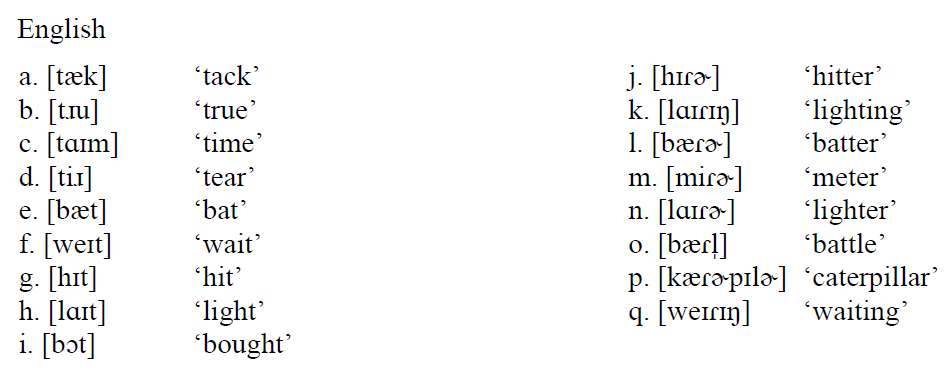
\includegraphics{../images/english_t_flap.png}
\end{figure}

\newpage

{\large Question 4}\\

Source: Week 2 Handout, Part II, Question 11\\

How would this word be transcribed?\\ Kathleen will likely ask a follow-up question about why you used a particular symbol.\\

<wealth>


\newpage

{\large Question 5}\\

Source: \\

What do the two signs below tell you about the phonological status of \underline{handshape} in ASL, and why?\\

\begin{figure}[H]
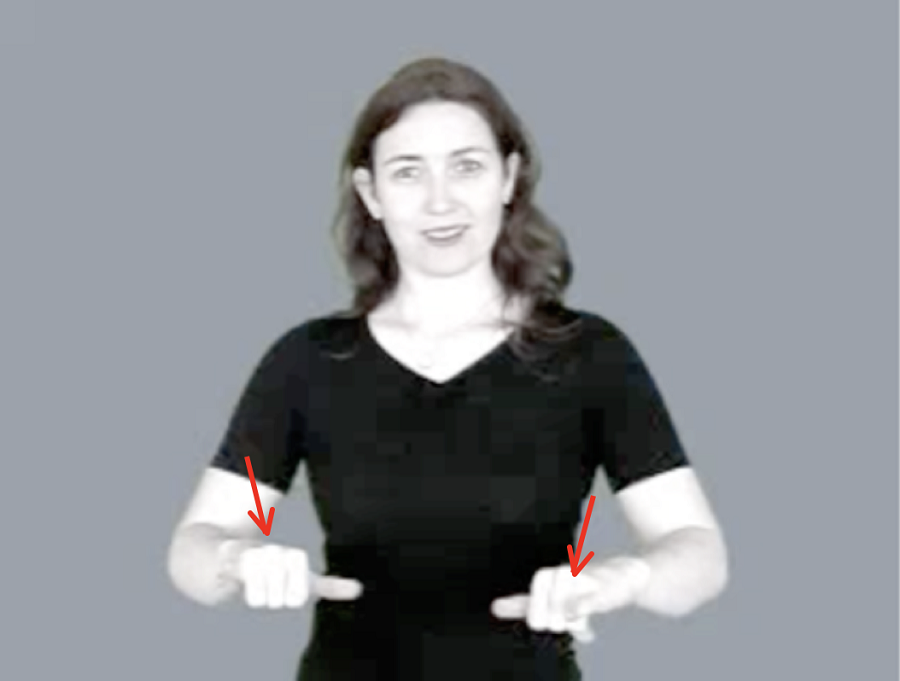
\includegraphics{../images/asl_stay.png}
\caption{STAY}
\end{figure}
\begin{figure}[H]
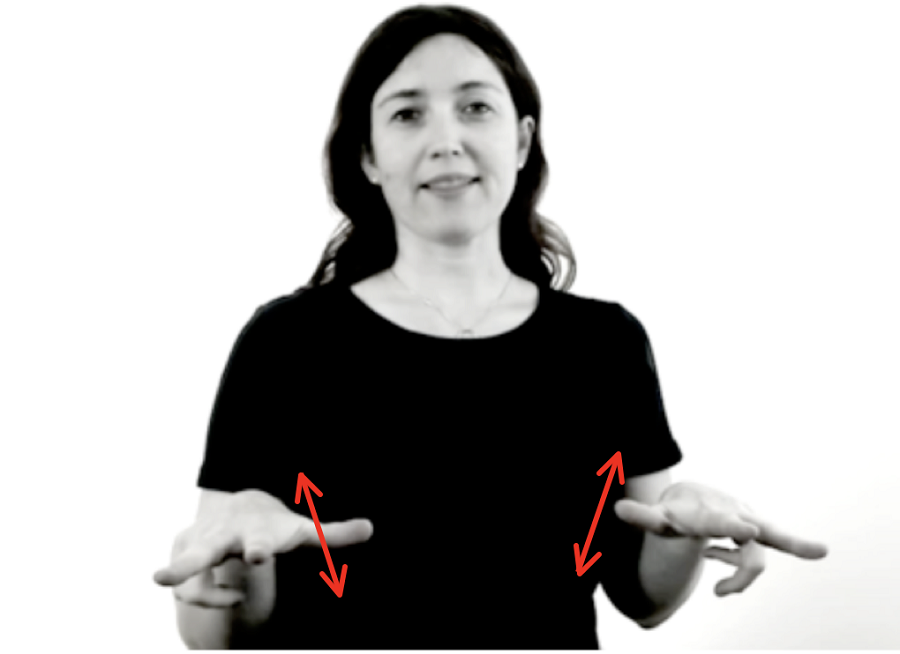
\includegraphics{../images/asl_awkward.png}
\caption{AWKWARD}
\end{figure}

\newpage

\begin{center}
\textbf{{\color{red}{\HUGE END OF EXAM}}}\\

\end{center}
\newpage

\begin{center}
\textbf{{\color{blue}{\HUGE START OF EXAM\\}}}

\textbf{{\color{blue}{\HUGE Student ID: 84480\\}}}

\textbf{{\color{blue}{\HUGE \\}}}

\end{center}
\newpage

{\large Question 1}\\

Source: Week 2 Handout, Part II, Question 11\\

How would this word be transcribed?\\ Kathleen will likely ask a follow-up question about why you used a particular symbol.\\

<toy>


\newpage

{\large Question 2}\\

Source: \\

Explain how you should use phonological features to combine these rules.\\

/pʰ/ → {[p]} / {[s]} \_\_\\/tʰ/ → {[t]} / {[s]} \_\_\\/kʰ/ → {[k]} / {[s]} \_\_

\begin{figure}[H]
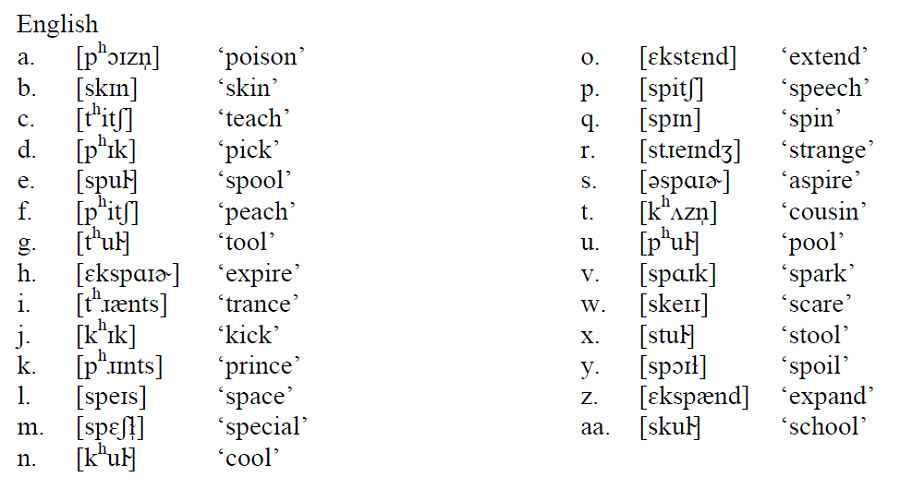
\includegraphics{../images/english_asp.png}
\end{figure}

\newpage

{\large Question 3}\\

Source: Week 3 Handout, Question 7\\

Is the symbol given a reasonable way to transcribe any of the sounds described below? If so, which one? If not, why not?\\

{[ʒ]}

\begin{itemize} \item voiceless palatal affricate \item voiced velar nasal \item voiceless glottal fricative \item voiced labiodental fricative \item voiced interdental fricative \item voiced palatal fricative \end{itemize}


\newpage

{\large Question 4}\\

Source: Quiz 4, Question 1\\

L$_X$ (Language X) has three vowels, [i], [a], and [u]. It has bi-syllabic roots like Kikuyu. It does not allow non-identical high vowels to co-occur. Of the following nine logically possible vocalic sequences, which ones should be unattested in L$_X$? Explain why.\\

\begin{itemize} \item {[i...i]} \item {[i...a]} \item {[i...u]} \item {[a...i]} \item {[a...a]} \item {[a...u]} \item {[u...i]} \item {[u...a]} \item {[u...u]} \end{itemize}


\newpage

{\large Question 5}\\

Source: \\

What do the two signs below tell you about the phonological status of \underline{handshape} in ASL, and why?\\

\begin{figure}[H]
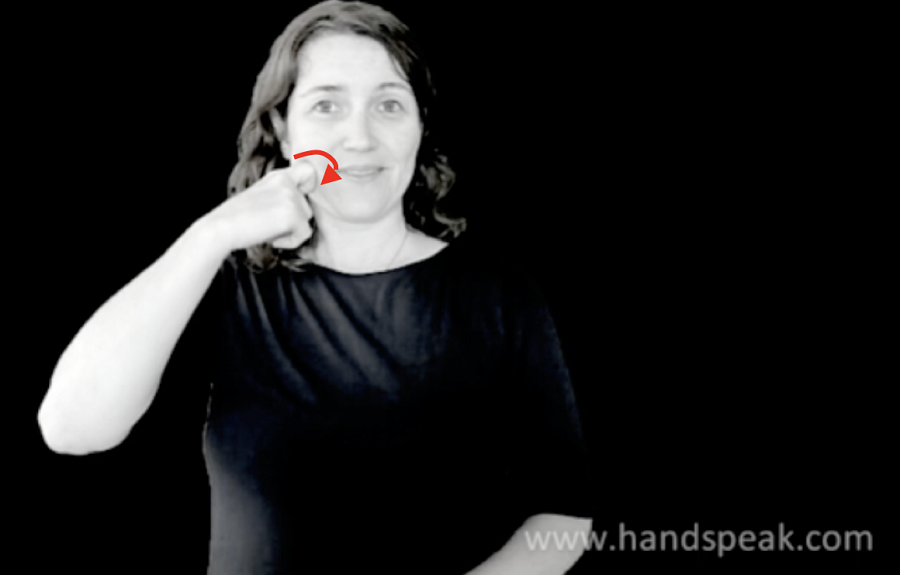
\includegraphics{../images/asl_apple.png}
\caption{APPLE}
\end{figure}
\begin{figure}[H]
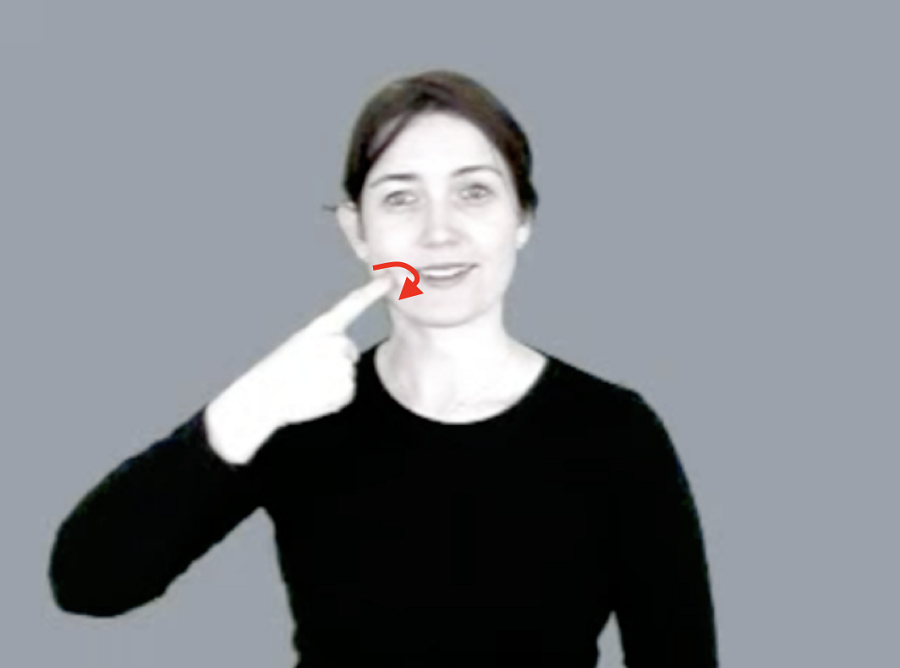
\includegraphics{../images/asl_candy.png}
\caption{CANDY}
\end{figure}

\newpage

\begin{center}
\textbf{{\color{red}{\HUGE END OF EXAM}}}\\

\end{center}
\newpage

\begin{center}
\textbf{{\color{blue}{\HUGE START OF EXAM\\}}}

\textbf{{\color{blue}{\HUGE Student ID: 85868\\}}}

\textbf{{\color{blue}{\HUGE \\}}}

\end{center}
\newpage

{\large Question 1}\\

Source: Week 3 Handout, Question 13\\

Explain why this image does or does not match the description.\\

\begin{itemize} \item A one-handed sign. \item Location: At the signer’s nose. \item Handshape: Starts with index finger extended; finger folds down into a “hook” shape during the sign; then straightens and repeats the folding. \item Movement: No movement other than the change in handshape. \end{itemize}

\begin{figure}[H]
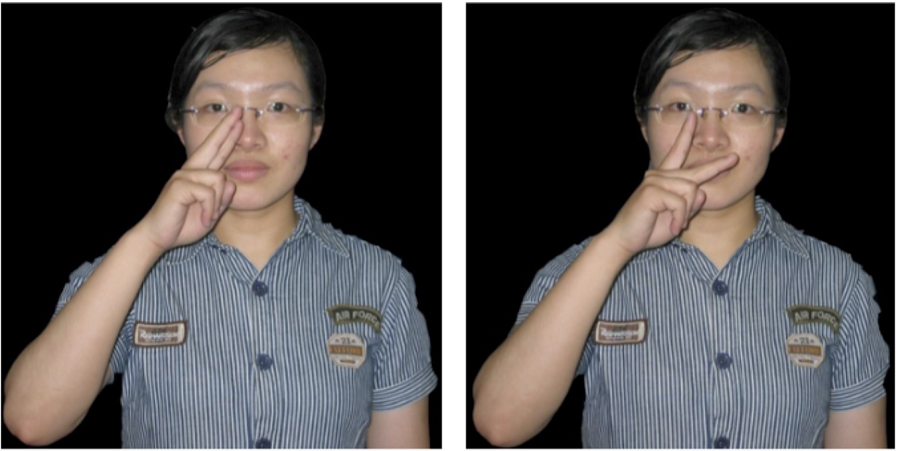
\includegraphics{../images/taiwansign_wrong.png}
\caption{WRONG}
\end{figure}

\newpage

{\large Question 2}\\

Source: Week 5 Handout, Question 5\\

Explain why looking for patterns with consonants and vowels is a more reasonable approach to pattern finding in this dataset than looking for patterns with respect to all of the individual sounds in Ukrainian.\\

\begin{figure}[H]
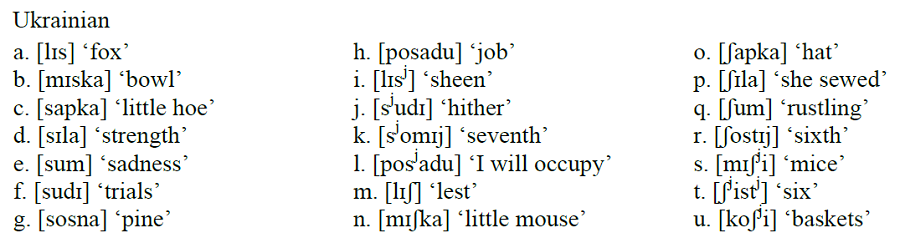
\includegraphics{../images/ukrainian.png}
\end{figure}

\newpage

{\large Question 3}\\

Source: Quiz 1, Question 10\\

Explain whether this word either does or does not have an [ʃ] sound in it, and why the spelling and pronunciation either do or do not align.\\

<meticulous>


\newpage

{\large Question 4}\\

Source: \\

Explain which sound should be removed to make this a natural class, and what the minimum set of features would be to describe the resulting natural class.\\

{[i]}, {[ɪ]}, {[ɛ]}, {[u]}, {[ʊ]}


\newpage

{\large Question 5}\\

Source: \\

What do the two signs below tell you about the phonological status of \underline{handshape} in ASL, and why?\\

\begin{figure}[H]
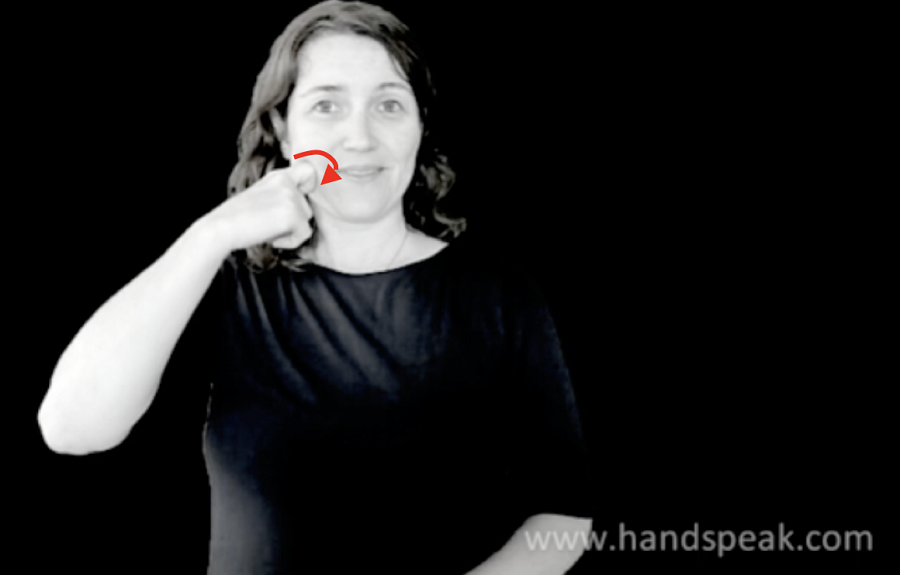
\includegraphics{../images/asl_apple.png}
\caption{APPLE}
\end{figure}
\begin{figure}[H]
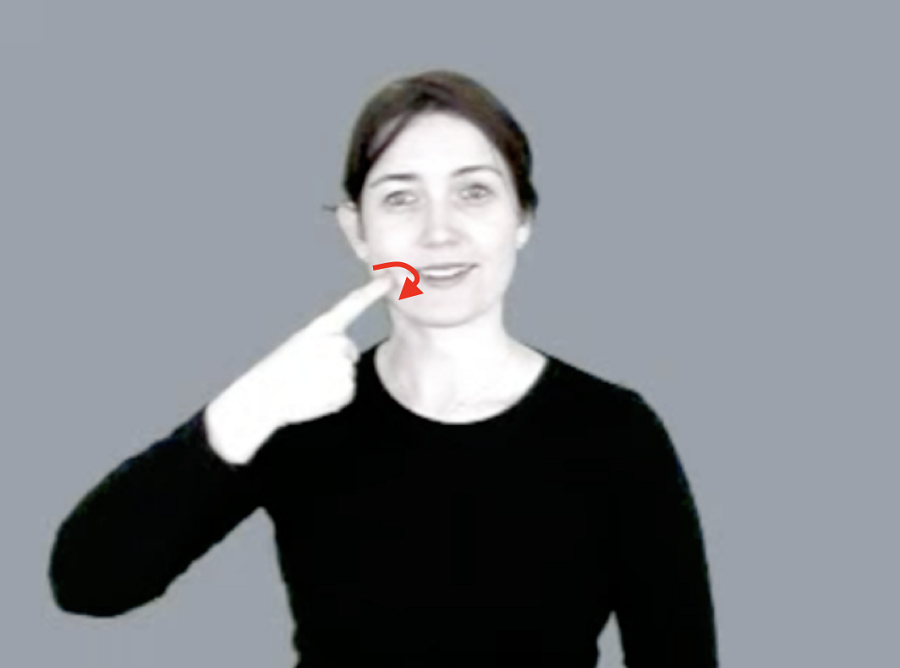
\includegraphics{../images/asl_candy.png}
\caption{CANDY}
\end{figure}

\newpage

\begin{center}
\textbf{{\color{red}{\HUGE END OF EXAM}}}\\

\end{center}
\newpage

\end{document}

